\documentclass[activite]{thedocument}
\usepackage{texmaths-boxes}
\startdatakeys
\source{}
\cycle{}
\competencesDuSocle{}
\connaissancesRequises{}
\competencesTravaillees{}
\enddatakeys
\begin{document}
\begin{center}
    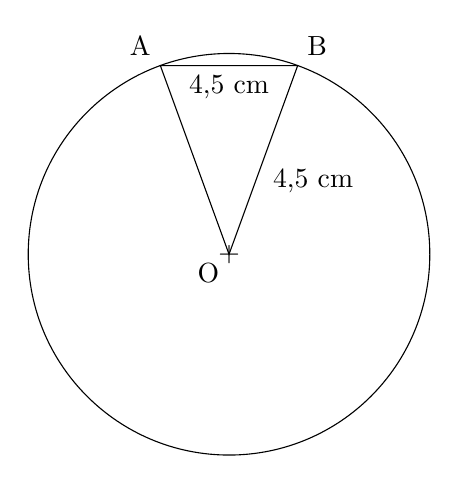
\begin{tikzpicture}[scale=0.85]
        \coordinate[label=below left:O](O)at(0,0);
        \coordinate[label=above left:A](A)at(110:3);
        \coordinate[label=above right:B](B)at(70:3);
        \draw node at (O){+};
        \path(A)--(B)node[below,midway]{4,5 cm};
        \path(O)--(B)node[below right,midway]{4,5 cm};
        \draw(A)--(B)--(O)--cycle;
        \draw(O)circle(3);
    \end{tikzpicture}
\end{center}\vskip50pt
\TableauRaisonnement scale=150pt;
\end{document}